\documentclass[tikz,border=8pt]{standalone}
\usepackage{amsmath}
\usepackage{pgfplots}
\usepgfplotslibrary{polar}
\usetikzlibrary{arrows.meta,calc}
\pgfplotsset{compat=1.18}
\definecolor{ink}{HTML}{17324D}
\definecolor{accent}{HTML}{0F766E}
\definecolor{gold}{HTML}{C28524}
\begin{document}
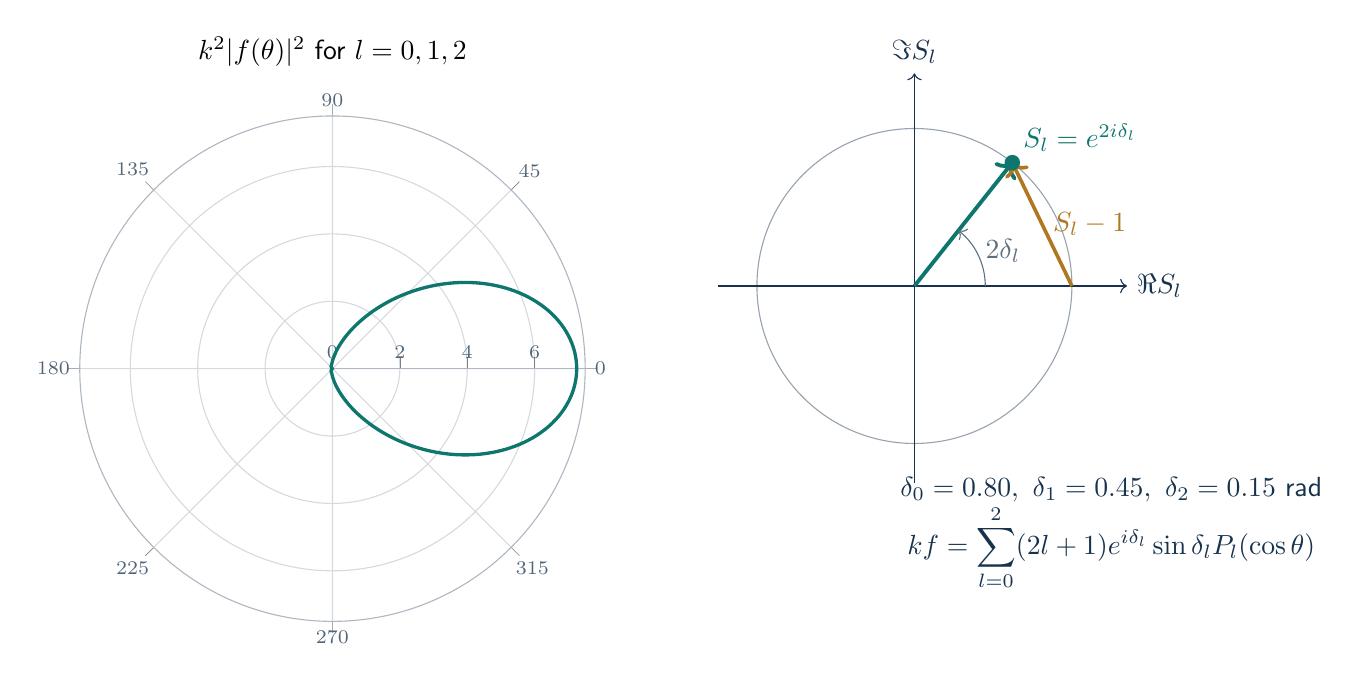
\begin{tikzpicture}[font=\sffamily]
 \begin{polaraxis}[
  at={(0,0)},anchor=west,width=8cm,height=8cm,
  title={$k^2|f(\theta)|^2$ for $l=0,1,2$},
  grid=both,grid style={ink!18},axis line style={ink!35},
  xtick={0,45,...,315},ytick={0,2,4,6},ymin=0,ymax=7.5,
  tick label style={font=\scriptsize,ink!75},
 ]
  \addplot[accent,very thick,domain=0:360,samples=721]
  {(
   (sin(45.8366)*cos(45.8366)+3*sin(25.7831)*cos(25.7831)*cos(x)
    +5*sin(8.5944)*cos(8.5944)*(3*cos(x)^2-1)/2)^2
   +(sin(45.8366)^2+3*sin(25.7831)^2*cos(x)
    +5*sin(8.5944)^2*(3*cos(x)^2-1)/2)^2
   )};
 \end{polaraxis}
 \begin{scope}[xshift=10.6cm,yshift=1.05cm,scale=2.0]
  \draw[ink!45] (0,0) circle (1);
  \draw[->,ink] (-1.25,0)--(1.35,0) node[right] {$\Re S_l$};
  \draw[->,ink] (0,-1.25)--(0,1.35) node[above] {$\Im S_l$};
  \def\twodelta{51.5662}
  \coordinate (One) at (1,0);
  \coordinate (Sl) at ({cos(\twodelta)},{sin(\twodelta)});
  \draw[accent,line width=1.4pt,->] (0,0)--(Sl) node[above right] {$S_l=e^{2i\delta_l}$};
  \draw[gold!90!black,line width=1.3pt,->] (One)--(Sl) node[midway,right] {$S_l-1$};
  \draw[->,ink!70] (.45,0) arc[start angle=0,end angle=\twodelta,radius=.45]
    node[pos=.58,right] {$2\delta_l$};
  \fill[accent] (Sl) circle (1.4pt);
 \end{scope}
 \node[ink,align=center] at (13.1,-2.1)
 {$\delta_0=0.80,\ \delta_1=0.45,\ \delta_2=0.15$ rad\\
  $\displaystyle kf=\sum_{l=0}^{2}(2l+1)e^{i\delta_l}\sin\delta_lP_l(\cos\theta)$};
\end{tikzpicture}
\end{document}
